\chapter{Eksperymenty}
W tej sekcji przedstawimy dwa środowiska testowe użyte do oceny zaproponowanych algorytmów dla decydenta zobowiązanego w modelach z dyskontowaniem quasi-hiperbolicznym. Te eksperymenty są możliwe do policzenia analitycznie, co pozwala na weryfikację poprawności implementacji oraz ocenę wydajności algorytmów. Dodatkowo przedstawimy eksperyment modelujący problem zarządzania zapasami rozbitka, w bardziej złożonym środowisku, którego nie będziemy rozwiązywać analitycznie, a jedynie zbadamy zachowanie algorytmów w praktyce, najpewniej uzyskując polityki suboptymalne. Wrócimy też do decydenta naiwnego, który był przedstawiony na wstępie i zobaczymy jak będzie się zachowywał w stosunku do decydenta zobowiązanego.
\section{Polityka próbkowania i kroki uczenia $\eta_n$, $\theta_n$}
W eksperymentach wykorzystujemy politykę próbkowania $\nu$ jako politykę losową, która wybiera każdą akcję mającą jakikolwiek sens z jednakowym prawdopodobieństwem w każdym stanie. Taka polityka zapewnia eksplorację całej przestrzeni stanów i akcji, co jest kluczowe dla skutecznego uczenia się w środowiskach MDP. \\
Na przykładzie kupowania produktu do magazynu, nie ma sensu wybierać akcji kupna większej ilości niż maksymalna pojemność magazynu minus aktualny stan zapasów. Wtedy dla magazynu o pojemności 4 w stanie posiadania 2 polityka próbkowania $\nu$ będzie wybierać akcje z zestawu $\{0, 1, 2\}$ z jednakowym prawdopodobieństwem $1/3$. \\
Kroki uczenia $\eta_n$ i $\theta_n$ ustawiamy zgodnie z warunkami Robbinsa-Monro przedstawionymi w poprzednich rozdziałach. W eksperymentach wykorzystujemy harmonogramy kroków uczenia w postaci:
\[
\eta_n = \frac{\eta_0}{(c + n)^{\kappa}},
\qquad
\theta_n = \frac{\theta_0}{(c + n)^{\lambda}},
\]
gdzie $c>0$ jest stałą zapobiegającą zbyt dużym krokom na początku (offset), a wykładniki spełniają
\[
\frac{1}{2} < \kappa < \lambda \le 1,
\]
co zapewnia warunki Robbinsa--Monro $\sum\limits_n \eta_n = \infty$, $\sum\limits_n \eta_n^2 < \infty$ (analogicznie dla $\theta_n$) oraz separację dwuskalową $\frac{\theta_n}{\eta_n} \to 0$.

Przy doborze tych hiperparametrów należy zachować kompromis. Jeżeli iloraz $\frac{\theta_n}{\eta_n}$ maleje zbyt wolno, separacja skal czasowych jest słaba i algorytm przez długi czas „miesza” oba procesy aktualizacji, co opóźnia stabilizację estymat. Z kolei zbyt szybki spadek $\frac{\theta_n}{\eta_n}$ sprawia, że skala wolna ($\theta_n$) uczy się bardzo zachowawczo, przez co zbieżność komponentu odpowiadającego za wartość quasi-hiperboliczną może być nadmiernie powolna.

\begin{figure}[htbp]
    \centering
    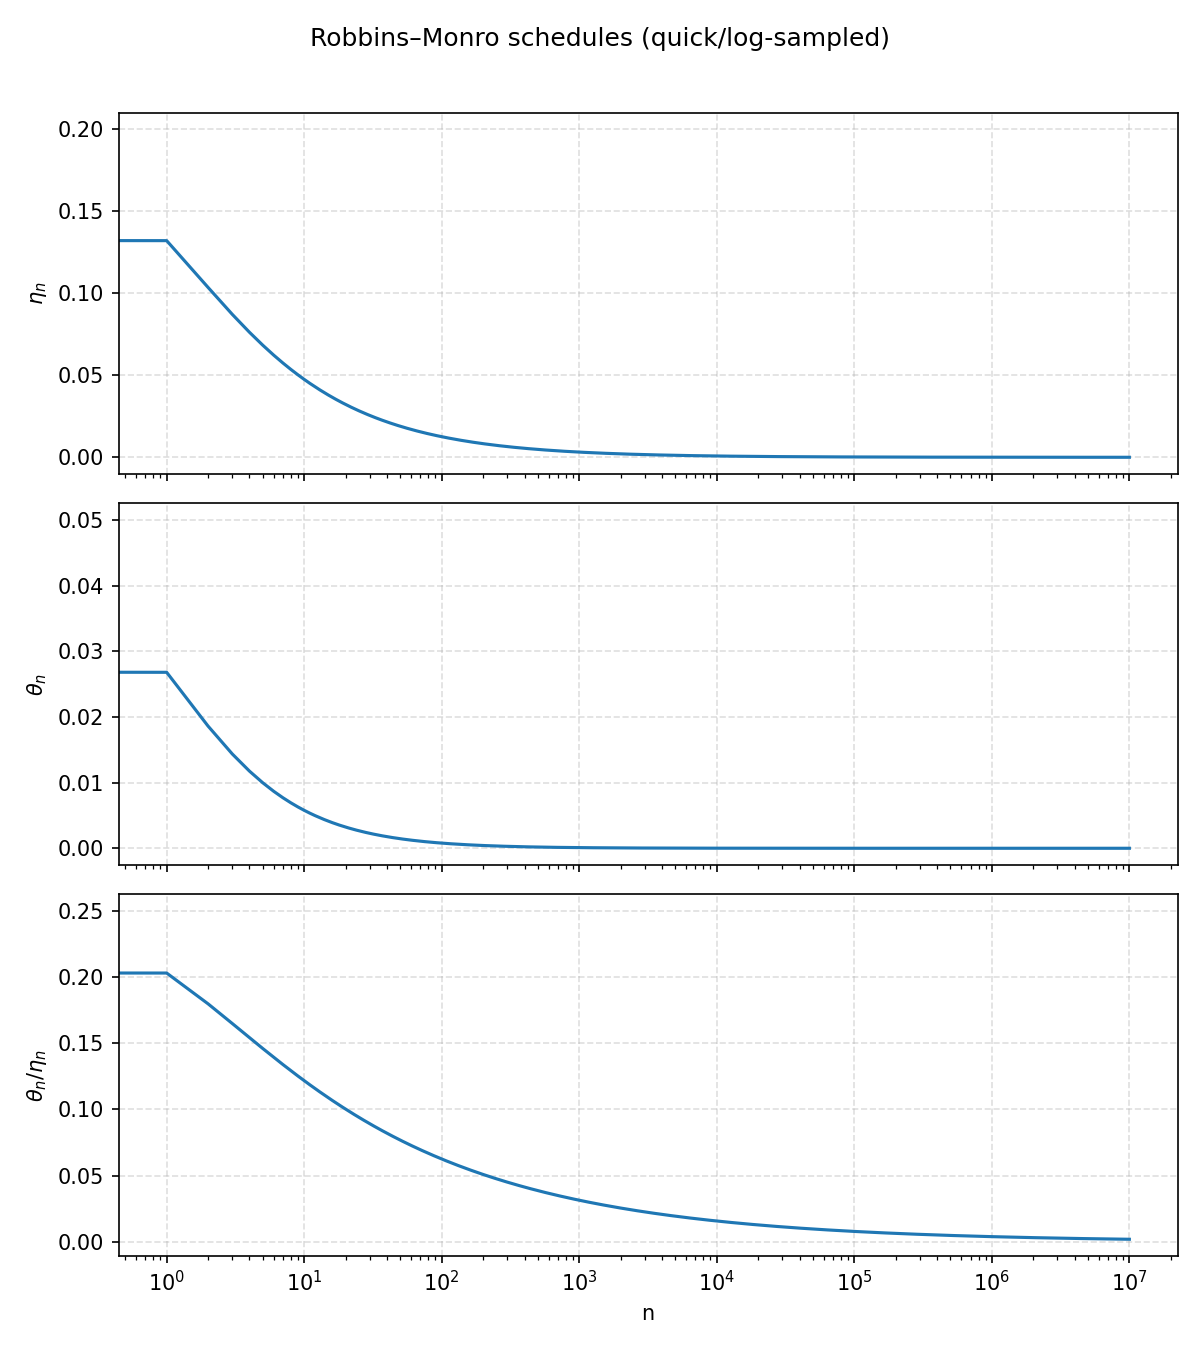
\includegraphics[width=0.7\textwidth]{../../plots/notebook_runs/robbins_monro_schedules_quick.png}
    \caption{Harmonogramy kroków uczenia $\eta_n$ i $\theta_n$ zgodne z warunkami Robbinsa-Monro dla $\eta_0 = 0.2,\kappa = 0.6, \theta_0 = 0.05, \lambda = 0.9$.}
    \label{fig:robbins-monro-schedules}
\end{figure}

\section{Środowiska testowe}

\subsection{Dwustanowy MDP z dyskontowaniem quasi-hiperbolicznym}

Pierwszym środowiskiem testowym jest prosty dwustanowy MDP, policzymy dla niego optymalną politykę dla decydenta zobowiązanego z dyskontowaniem quasi-hiperbolicznym oraz porównamy ją z optymalną polityką dla dyskontowania wykładniczego. Przeprowadzimy 
\subsubsection{Definicja modelu}

\begin{figure}[htbp]
    \centering
    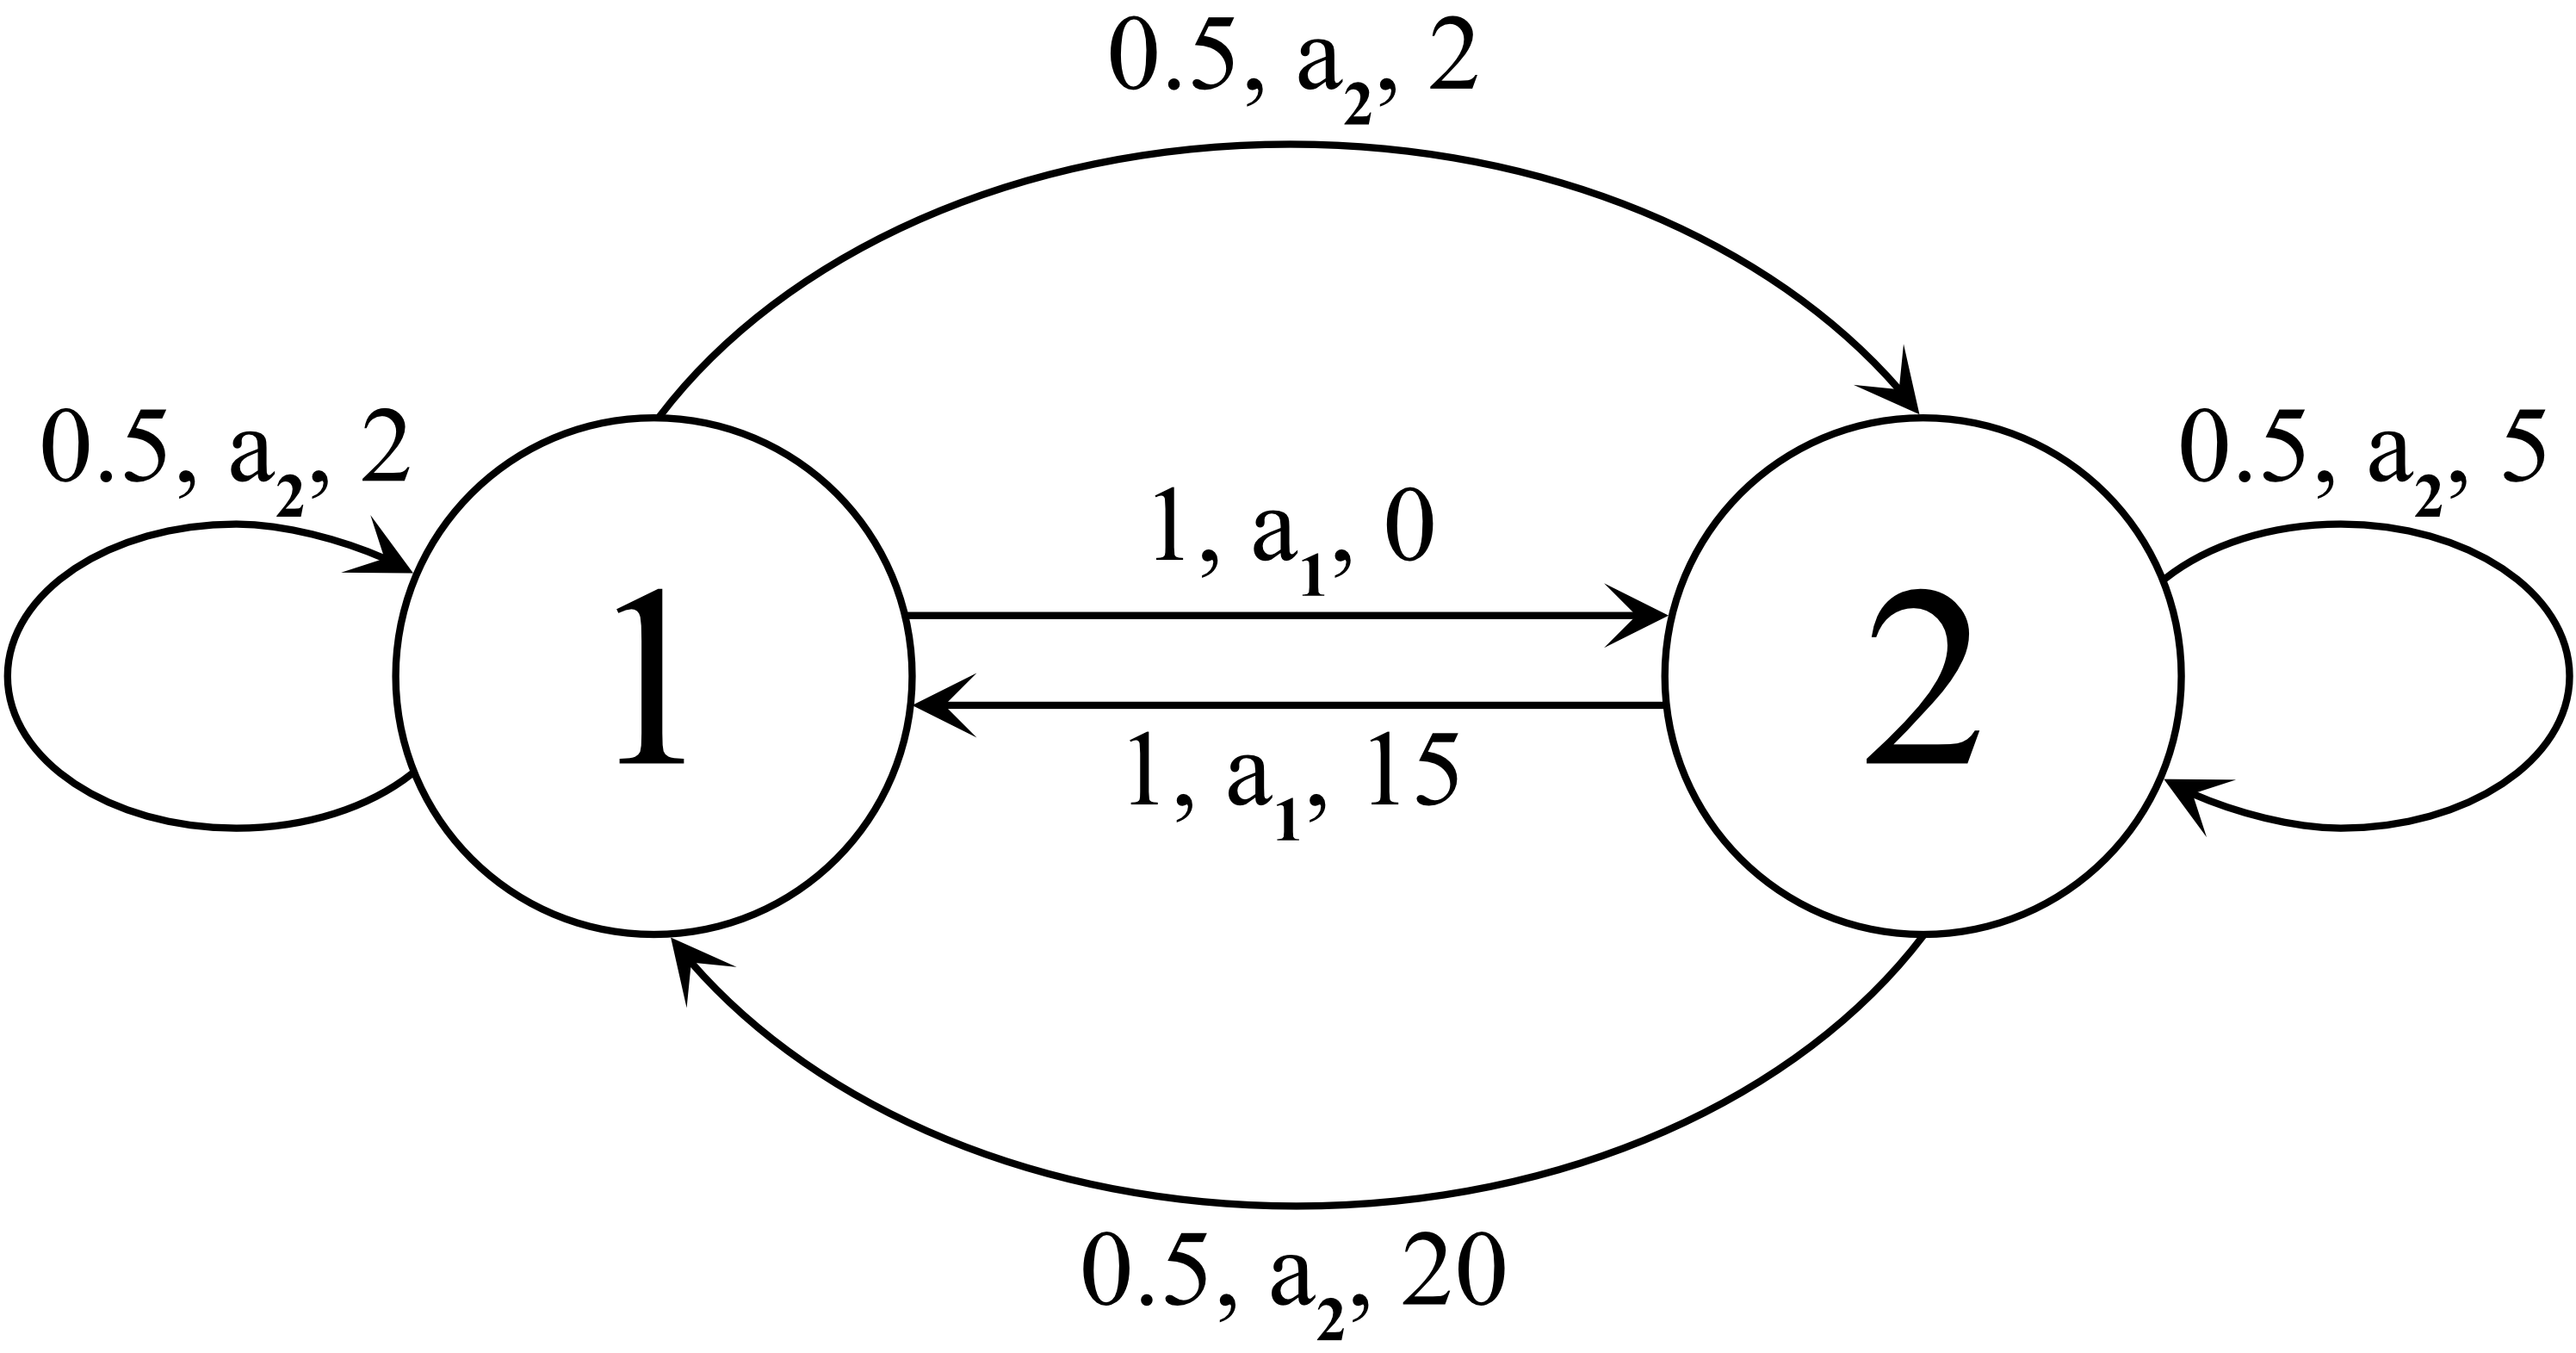
\includegraphics[width=0.7\textwidth]{fig/example1.png}
    \caption{Struktura dwustanowego MDP: stany (1, 2), akcje ($a_1, a_2$), nagrody i przejścia probabilistyczne w formacie $q(s' \mid s, a), a_n, r(s, a_n).$}
    \label{fig:two-state-mdp}
\end{figure}

Rozpatrujemy MDP $M = (S, A, q, r, \alpha, \beta)$ z:
\begin{itemize}
\item Przestrzeni stanów: $S = \{1, 2\}$
\item Przestrzeni akcji: $A = \{a_1, a_2\}$
\item Funkcja nagrody: $r(1, a_1) = 0$, $r(1, a_2) = 2$, $r(2, a_1) = 5$, $r(2, a_2) = 20$ dla 
\item Przejścia:
\begin{align}
q(2 \mid 1, a_1) &= 1.0 \quad \text{(deterministyczne)} \\
q(1 \mid 1, a_2) &= 0.5, \quad q(2 \mid 1, a_2) = 0.5 \\
q(1 \mid 2, a_1) &= 0.5, \quad q(2 \mid 2, a_1) = 0.5 \\
q(1 \mid 2, a_2) &= 0.5, \quad q(2 \mid 2, a_2) = 0.5
\end{align}
\end{itemize}

\subsubsection{Interpretacja}

Model ilustruje klasyczną niespójność czasową: w stanie 1 akcja $a_1$ prowadzi deterministycznie do stanu 2 (gdzie czekają duże nagrody), podczas gdy $a_2$ daje małą nagrodę natychmiast. Dla agenta niezaangażowanego (present-biased) akcja $a_2$ może być bardziej atrakcyjna ze względu na natychmiastową nagrodę.


\section{Metryki oceny}

Do oceny algorytmów używamy następujących metryk:
\begin{itemize}
\item Zbieżność do optymalnej polityki
\item Czas obliczeniowy
\item Stabilność numeryczna
\item Wrażliwość na parametry
\end{itemize}

\section{Wyniki eksperymentów}

\subsection{Porównanie z metodami tradycyjnymi}

Porównujemy proponowane algorytmy z tradycyjnymi metodami dla dyskontowania wykładniczego.

\subsection{Wpływ parametrów}

Analizujemy wpływ parametrów $\sigma$ i $\gamma$ na właściwości algorytmów.

\section{Dyskusja wyników}

Interpretujemy otrzymane wyniki w kontekście teorii i praktycznych zastosowań.